\documentclass[conference]{IEEEtran}
\IEEEoverridecommandlockouts
% The preceding line is only needed to identify funding in the first footnote. If that is unneeded, please comment it out.
\usepackage{cite}
\usepackage{amsmath,amssymb,amsfonts}
\usepackage{algorithmic}
\usepackage{graphicx}
\usepackage{textcomp}
\usepackage{xcolor}
\def\BibTeX{{\rm B\kern-.05em{\sc i\kern-.025em b}\kern-.08em
    T\kern-.1667em\lower.7ex\hbox{E}\kern-.125emX}}
\begin{document}

\title{Assumption of Bitcoin Regulation Using Extra Basic Data Structures \\
}

\author{\IEEEauthorblockN{1\textsuperscript{st} Liu Feng}
\IEEEauthorblockA{\textit{ECE Department} \\
\textit{Stevens Institute of Technology}\\
Hoboken, USA \\
fliu17@stevens.edu}
\and
\IEEEauthorblockN{1\textsuperscript{st} Wu Siyang}
\IEEEauthorblockA{\textit{ECE Department} \\
	\textit{Stevens Institute of Technology}\\
	Hoboken, USA \\
swu32@stevens.edu}
\and
\IEEEauthorblockN{1\textsuperscript{st} Xu Xiangyang}
\IEEEauthorblockA{\textit{ECE Department} \\
	\textit{Stevens Institute of Technology}\\
	Hoboken, USA \\
xxu46@stevens.edu}
}

\maketitle

\begin{abstract}
Bitcoin is a decentralized digital currency without any banks or administrators. Since Bitcoin can be sent from user to user with no intermediaries, we decide to conceive a manner for regulating it. After the study about Libra (a cryptocurrency which is similar with Bitcoin), we use some basic data structures (Hash Table and Array List) as the assistance and apply the SHA256 algorithm in our work. 
\end{abstract}

\begin{IEEEkeywords}
Bitcoin, regulating, Libra, data structures, SHA256
\end{IEEEkeywords}

\section{Introduction}
Bitcoin is a collection of concepts and technologies that form the basis of a digital money ecosystem.  Bitcoin is created through a process called "mining," which involves competing to find solutions to a mathematical problem while processing bitcoin transactions and it also has the protocol, which includes built-in algorithms that regulate the mining function across the network. Due to bitcoin’s diminishing rate of issuance, more and more company start to make their own cryptocurrency to take over Bitcoin’s status. [1]

Recently, there comes another virtual currency which is Libra, it is the project for which social media giant Facebook released the concept paper on 18 June 2019. To regulate Libra, Facebook lets Libra commit to open access to the blockchain, and open infrastructure, given that “open access ensures low barriers to entry and innovation and encourages healthy competition that benefits consumers.” [2]

In a degree, Bitcoin is similar with Libra. Even though the real incentive for Bitcoin was to avoid regulatory agencies, we still propose to use basic data structures and apply an algorithm to make it possible for regulation of Bitcoin.

\section{FUNCTION WITH DIAGRAMS}
\subsection{Encode the Trade Information by applying SHA-256 algorithm (Feng Liu)}
People like to use Bitcoin because it can protect user’s privacy. On the contrary, the server will ruin this advantage in that user must offer their corresponding information. To make a remedy for this issue, we plan to encode the trade information. By doing that, we can not only protect user’s privacy but also prevent the database from being stolen by lawbreakers. That means the user name is not the real name of the user. Therefore, the user’s name in the transaction’s information broadcasted will not be related to the real user. All the user’s real information is saved and maintained in our server. So it is impossible to reach any real users on the network by using encoded user’s name.

From the server we have, we can get the information of Miner, Giver and Payee and apply the algorithm of SHA-256 to encode them.

In SHA-256 algorithm, the 64 constants used are similar with the 8 hash initial values. These constants are obtained by taking the first 32 bits of the fractional part of the cube root of the first 64 prime numbers in the natural number.

The pre-processing in the SHA256 algorithm is to add the required information after the message you want to hash. And it is divided into two steps: additional padding bits and additional length. As for the first step: append the bit '1' to the message and append k bits '0' where k is the minimum number (greater or equals to 0). And the resulting message length (in bits) is congruent to 448 (mod 512). And as for the second step: append length of message (before pre-processing), in bits, as 64-bit big-endian integer.

Then we need to break the message (user’s information) into 512-bit blocks for encryption.

\begin{figure}[ht]
	\centering
	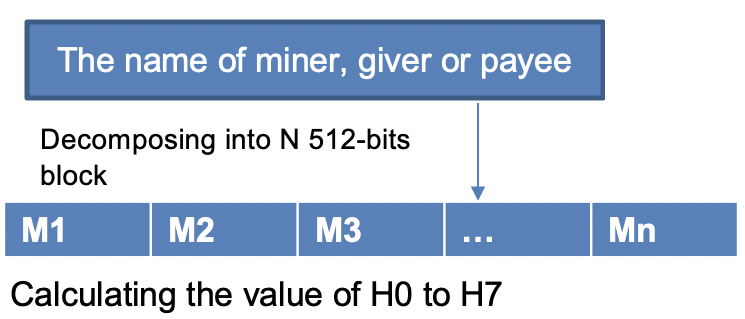
\includegraphics[scale=0.3]{fig2.png}
	\caption{Breaking the messge (user name)}
	\label{fig:label}
\end{figure}


\section{PSEUDO CODE}
\subsection{Main Loop Part}
Suppose the message M can be decomposed into n blocks, so all the algorithm needs to do is complete n iterations, and the result of n iterations is the final hash value, which is a 256-bit digital digest. In the first iteration, the initial value of the mapping is set to the 8 hash initial values introduced earlier, as shown in the following code:

\section{CONCLUSION}
Bitcoin is a decentralized cryptocurrency and has been criticized for its use in illegal transactions, its high electricity consumption, price volatility, and thefts from exchanges. Since the property of the blockchain of Bitcoin, it is very hard to modify any information of any transaction. However, if we use other extra basic data structures as a support to get an access to its blockchain just like what Facebook did to Libra, it will be regulated so how. In fact, it is impossible to fulfil the regulation of the Bitcoin and we hope our assumption can be applied to Bitcoin’s system one day.

\section{CONTRIBUTION}
In this work, Siyang Wu conceived the whole idea and composed the major part of this paper. Feng Liu has searched the algorithm for hash function and analyzed it. Xiangyang Xu has read the paper of the Libra and studied the property of the data structures we use.  

\begin{thebibliography}{00}
\bibitem{b1} Andreas Antonopolous (2014). Mastering bitcoin: Programming the Open Blockchain
\bibitem{b2} Zetzsche D.A, Buckley R.P, Arner D.W (2019). Regulating LIBRA: The Transformative Potential of Facebook’s Cryptocurrency and Possible Regulatory Responses
\bibitem{b3} Cormen, Thomas H.; Leiserson, Charles E.; Rivest, Ronald L.; Stein, Clifford (2009). Introduction to Algorithms (3rd ed.). Massachusetts Institute of Technology. pp. 253–280. ISBN 978-0-262-03384-8.
\end{thebibliography}
\end{document}


